\documentclass[conference]{IEEEtran}
%\IEEEoverridecommandlockouts
% The preceding line is only needed to identify funding in the first footnote. If that is unneeded, please comment it out.
%Template version as of 6/27/2024

\usepackage{booktabs}
\usepackage{cite}
\usepackage{amsmath,amssymb,amsfonts}
\usepackage{algorithmic}
\usepackage{graphicx}
\usepackage{textcomp}
\usepackage{xcolor}
\def\BibTeX{{\rm B\kern-.05em{\sc i\kern-.025em b}\kern-.08em
    T\kern-.1667em\lower.7ex\hbox{E}\kern-.125emX}}
    
\begin{document}

\title{Clasificación de Plantaciones de Palma de Aceite en Colombia utilizando Deep Learning y Datos Satelitales de Sentinel-1 y Sentinel-2}

\author{\IEEEauthorblockN{Kevin Steven Gamez Abril}
\IEEEauthorblockA{\textit{Departamento de Ingeniería de Sistemas y Computación} \\
\textit{Universidad de los Andes}\\
Bogotá, Colombia\\
ks.gamez@uniandes.edu.co}
\and
\IEEEauthorblockN{Haydemar María Nuñez Castro}
\IEEEauthorblockA{\textit{Departamento de Ingeniería de Sistemas y Computación} \\
\textit{Universidad de los Andes}\\
Bogotá, Colombia\\
h.nunez@uniandes.edu.co}
\and
\IEEEauthorblockN{Andrés Oswaldo Calderón Romero}
\IEEEauthorblockA{\textit{Deparment of Computer Science and Engineering} \\
\textit{University of California}\\
Riverside, USA \\
acald013@ucr.edu}
\and
\IEEEauthorblockN{Rocío Sierra Ramírez}
\IEEEauthorblockA{\textit{Departamento de Ingeniería Química y de Alimentos} \\
\textit{Universidad de los Andes}\\
Bogotá, Colombia\\
rsierra@uniandes.edu.co}
}

\maketitle

\begin{abstract}
Este estudio presenta un modelo avanzado basado en Deep Learning para la clasificación de plantaciones de palma de aceite en Colombia, utilizando datos satelitales de Sentinel-1 y Sentinel-2. Ante la creciente demanda de alimentos y los desafíos del cambio climático, el enfoque propuesto mejora la gestión agrícola mediante la integración de datos radar y ópticos. El modelo implementado, basado en la arquitectura DeepLabV3+ con MobileNet V3 y ResNet50, emplea estrategias de transferencia de aprendizaje y ajuste fino para optimizar su rendimiento. La metodología comprende tres fases: modelado, implementación y validación, destacándose por una precisión global del 98.37\%. Este trabajo subraya la eficacia del Deep Learning en comparación con métodos tradicionales, superando limitaciones como la cobertura de nubes y resolviendo tareas complejas de segmentación de imágenes. Los resultados demuestran su aplicabilidad práctica en la gestión de cultivos, sugiriendo futuras mejoras para incluir plantaciones jóvenes y explorar otros tipos de cultivos y regiones geográficas.
\end{abstract}

\begin{IEEEkeywords}
Deep Learning, Clasificación de cultivos, Imágenes satelitales, Sentinel-1 y Sentinel-2, Agricultura de precisión.
\end{IEEEkeywords}


\section{Introducción}
La agricultura moderna enfrenta retos como el aumento de la demanda alimentaria debido al crecimiento poblacional, el cambio climático y el agotamiento de recursos naturales \cite{thayer2020}. Esto resalta la necesidad de optimizar el uso de la tierra para reducir el impacto ambiental y maximizar beneficios socioeconómicos. Los datos satelitales permiten mapear terrenos agrícolas, gestionar eficientemente recursos críticos como agua y fertilizantes, y monitorear la salud de los cultivos, mejorando la productividad \cite{boryan2011}.

Tradicionalmente, la identificación y monitoreo de cultivos dependían de observaciones de campo, un proceso intensivo y propenso a errores. Recientemente, imágenes aéreas capturadas por vehículos no tripulados han facilitado este proceso, proporcionando datos valiosos para la toma de decisiones agrícolas \cite{hu2021}. Las imágenes satelitales han sido ampliamente usadas para clasificar cultivos debido a su riqueza informativa.

Este trabajo propone un modelo de clasificación de cultivos basado en técnicas de Deep Learning, utilizando composiciones de bandas de imágenes satelitales. Primero, se analizará el estado del arte sobre el uso de Deep Learning para la identificación de zonas cultivadas, evaluando enfoques existentes y áreas de mejora. Además, se identificarán características relevantes de las imágenes que mejoren la clasificación. Se implementarán estrategias de transferencia de aprendizaje y ajuste fino (Fine-tuning) para aprovechar modelos preentrenados.

El modelo se aplicará a una región específica de Colombia y se comparará con métodos tradicionales basados en índices de vegetación, destacando las ventajas del enfoque de Deep Learning. La metodología se divide en tres fases: modelado, incluyendo la selección de arquitectura y preprocesamiento de imágenes de Sentinel 1 y Sentinel 2 \cite{descals2021}; implementación, enfocada en el entrenamiento y prueba de modelos preentrenados; y validación, que evaluará métricas de desempeño y analizará limitaciones del modelo para imágenes representativas del territorio colombiano.

\section{Revisión de la literatura}

El uso de técnicas de Deep Learning en el análisis de imágenes satelitales ha revolucionado la agricultura, convirtiéndola en una herramienta clave para la gestión y planificación agrícola. Estas tecnologías han mejorado significativamente la precisión en la predicción del rendimiento de cultivos y biomasa, facilitando decisiones basadas en datos y optimizando recursos.

Un análisis exhaustivo de 150 estudios \cite{victor2022} identificó cinco tareas principales donde la aplicación de Deep Learning podría traer beneficios: uso y cobertura del suelo, salud del suelo, fisiología de las plantas, daño a los cultivos y predicción del rendimiento. El estudio concluye que los métodos de Deep Learning superan a los tradicionales en la mayoría de las tareas, salvo en la predicción del rendimiento, donde los modelos LSTM muestran un rendimiento comparable a Random Forest. Este hallazgo subraya la importancia de disponer de conjuntos de datos de referencia públicos para una comparación efectiva entre estudios.

\subsection{Optimización de la Agricultura con Deep Learning}
El Deep Learning ha emergido como una herramienta clave para optimizar prácticas agrícolas mediante el análisis avanzado de datos satelitales. Su capacidad para procesar grandes volúmenes de información y abordar problemas complejos ha permitido mejorar la precisión en la estimación de rendimientos, superar limitaciones tradicionales y adaptarse a diversas condiciones geográficas. A continuación, se destacan ejemplos representativos que ilustran cómo estas técnicas están transformando la agricultura.

Por ejemplo, la estimación del rendimiento del café en Brasil mediante Deep Learning, combinado con modelos de regresión y análisis de imágenes satelitales, ha demostrado ser eficaz para anticipar la variabilidad espacial en mapas de rendimiento, apoyando la planificación agrícola \cite{martello2022}. Además, la escalabilidad del Deep Learning destacó en un estudio que utilizó datos geográficos y meteorológicos para estimar rendimientos de cinco cultivos principales en Brasil, mostrando su adaptabilidad a diversas condiciones agrícolas \cite{cunha2020}.

Aunque las imágenes satelitales suelen tener limitaciones en su resolución espacial, su resolución espectral superior permite el uso de algoritmos \textit{per-píxel}, mejorando el rendimiento en comparación con enfoques tradicionales \cite{victor2022}.  Métodos como las redes neuronales convolucionales (CNNs), aplicados a datos temporales y secuenciales, han abordado desafíos como la cobertura de nubes. En este contexto, las imágenes SAR de satélites como Sentinel-1 han mostrado mejores resultados al penetrar nubes en comparación con imágenes ópticas.

Para estudios sobre el uso del suelo, la combinación de datos de Sentinel-1, Sentinel-2 y Landsat-8 ha demostrado mejorar significativamente el rendimiento en comparación con el uso de una sola fuente.

\subsection{Casos de Estudio en Agricultura con Deep Learning}

A continuación, se presentan diversos casos de estudio que aplican técnicas de Deep Learning para clasificar diferentes tipos de cultivos. La Tabla \ref{tab:case_studies} resume los principales hallazgos de cada caso.

\begin{itemize}

    \item \textit{Coffee-Yield Estimation Using High-Resolution Time-Series Satellite Images and Machine Learning:} En este estudio \cite{martello2022}, se utilizó aprendizaje automático y datos de imágenes de alta resolución (PlanetScope) para predecir el rendimiento del café en Minas Gerais, Brasil. Se implementaron modelos Random Forest y regresión lineal múltiple, logrando un coeficiente de determinación ($R^2$) de 0.93 para la validación, destacando la precisión en el monitoreo de la variabilidad espacial.

    \item \textit{Corn Biomass Estimation by Integrating Remote Sensing and Long-Term Observation Data Based on Machine Learning Techniques:} En \cite{geng2021} se estimó la biomasa del maíz en la cuenca del río Heihe, China, utilizando datos MODIS y modelos como Random Forest, SVM y XGBoost. El modelo XGBoost obtuvo el mejor rendimiento ($R^2 = 0.78$, RMSE = 2.86 t/ha).

    \item \textit{Estimating Crop Yields with Remote Sensing and Deep Learning:} \cite{cunha2020} propusieron un modelo basado en Deep Learning para predecir rendimientos de cultivos en Brasil. Este modelo utilizó coordenadas geográficas, datos meteorológicos y del suelo, mostrando alta escalabilidad con datos limitados.

    \item \textit{Forecasting Crop Yield with Deep Learning-Based Ensemble Model:} \cite{divakar2022} emplearon un modelo basado en LSTM y ConvLSTM para predecir el rendimiento de cultivos en Estados Unidos e India. Con un coeficiente $R^2$ de 0.73 para la soja y 0.49 para el arroz, destacaron la eficiencia del modelo con menos parámetros.

    \item \textit{Forecasting Sunflower Grain Yield Using Remote Sensing Data:} \cite{debaeke2023} utilizaron datos de teledetección en Francia para predecir el rendimiento del girasol, combinando índices de vegetación como GAI\footnote{Green Area Index} y GAD\footnote{Growth Accumulation Dynamics} en modelos como Random Forest y regresiones polinómicas, logrando mejorar las predicciones a nivel de campo.

    \item \textit{High-Resolution Global Map of Smallholder and Industrial Closed-Canopy Oil Palm Plantations:} \cite{descals2021} mapearon plantaciones de palma aceitera usando modelos avanzados de aprendizaje profundo diseñados para segmentación semántica aplicado a imágenes Sentinel, obteniendo una precisión superior 98\%.

    \item \textit{A Systematic Review of the Use of Deep Learning in Satellite Imagery for Agriculture:} Se destaca \cite{victor2022} donde se revisaron 150 estudios de Deep Learning aplicados a imágenes satelitales, identificando tareas clave como clasificación del uso del suelo, fisiología de plantas y predicción de rendimientos.
    
    \item \textit{Machine Learning in Precision Agriculture: A Survey on Trends, Applications and Evaluations Over Two Decades:} Igualmente, \cite{condran2022} analiza cómo las técnicas de aprendizaje automático se han integrado en la agricultura de precisión en los últimos 20 años, evaluando aplicaciones, efectividad y tendencias emergentes. Es un recurso clave para entender la evolución y el estado actual de estas tecnologías.

\end{itemize}

\begin{table*}[t]
        \centering
        \caption{Resumen de casos de estudio en agricultura con Deep Learning}\label{tab:case_studies}
        \begin{tabular}{c c p{4.5cm} p{5.25cm}}
            \toprule
            \textbf{Referencia} & \textbf{Ubicación} & \textbf{Métodos y Modelos} & \textbf{Resultados Clave} \\ 
            \midrule
            \cite{martello2022} & Minas Gerais, Brasil & Random Forest, Regresión Lineal Múltiple, imágenes PlanetScope & $R^2 = 0.93$, alta precisión en variabilidad espacial \\ 
            \cite{geng2021} & Cuenca del río Heihe, China & MODIS, Random Forest, SVM, XGBoost & XGBoost: $R^2 = 0.78$, RMSE = 2.86 t/ha \\ 
            \cite{cunha2020} & Brasil & Coordenadas geográficas, datos meteorológicos y del suelo & Modelo escalable con datos limitados \\ 
            \cite{divakar2022} & EE.UU. e India & LSTM, ConvLSTM, datos MODIS y NASA-USDA & Soja: $R^2 = 0.73$, Arroz: $R^2 = 0.49$ \\ 
            \cite{debaeke2023} & Francia & GAI, GAD, Random Forest, regresiones polinómicas & Mejoras significativas en predicciones de rendimiento \\ 
            \cite{descals2021} & Global & Segmentación semántica sobre imágenes Sentinel & Precisión global $>$98\% en clasificación de palma aceitera \\ 
            \cite{victor2022} & Global & Revisión de 150 estudios de Deep Learning aplicados a imágenes satelitales & Identifica tareas clave: uso del suelo, fisiología de plantas, predicción de rendimientos \\ 
            \cite{condran2022} & Global & Revisión de estudios de dos décadas sobre machine learning y agricultura de precisión & Recopila el impacto del aprendizaje automático en la agricultura de precisión en los últimos 20 años. \\ 
            \bottomrule
        \end{tabular}
\end{table*}

\subsection{Tendencias Futuras y Potencial del Deep Learning en Agricultura}

El Deep Learning ha transformado significativamente la agricultura, mejorando la precisión en la estimación de rendimientos y biomasa de cultivos como café, maíz y palma de aceite. La integración de algoritmos avanzados, como CNN y RNN, con datos de teledetección ha facilitado predicciones oportunas y eficientes para la gestión de recursos agrícolas \cite{condran2022}.

El uso de imágenes satelitales se ha consolidado como una herramienta clave, permitiendo monitorear la salud del suelo, la fisiología de las plantas y evaluar daños en cultivos mediante índices espectrales. La comunidad científica destaca la necesidad de benchmarks públicos y métodos estandarizados para validar modelos y comparar resultados.

Para superar desafíos como la baja resolución espacial y las interferencias atmosféricas, se están desarrollando técnicas que maximizan el uso de los datos disponibles. Las innovaciones en Deep Learning prometen aplicaciones prácticas como la detección temprana de enfermedades, la optimización del uso del agua y la gestión de nutrientes, contribuyendo así a la sostenibilidad agrícola \cite{sepulveda2020}.

La colaboración interdisciplinaria entre agrónomos, científicos de datos y especialistas en teledetección es esencial para desarrollar soluciones integradas que impulsen la innovación en este campo en constante evolución \cite{nasa_arset_2023}.

\subsection{Ventajas y Desafíos}

El uso combinado de imágenes de Sentinel-1 (radar SAR) y Sentinel-2 (multi-espectrales) mejora significativamente la clasificación de cultivos, superando limitaciones como la cobertura de nubes. Sin embargo, persisten desafíos relacionados con la resolución espacial y la necesidad de benchmarks públicos que faciliten la comparación entre estudios.

\section{Preliminares}

\subsection{Convolución Atrous}

La convolución \textit{atrous} o dilatada es una variante de la convolución tradicional en redes neuronales convolucionales (CNNs) que inserta espacios entre los elementos del kernel, ampliando el campo receptivo sin aumentar el número de parámetros \cite{chen2017}. Esto permite capturar características a mayor escala, siendo especialmente útil en tareas como la segmentación semántica, donde se requiere una perspectiva global de la entrada. Además, la convolución \textit{atrous} facilita una extracción de características más densa en las capas profundas sin comprometer la resolución espacial. Esto se logra ajustando la tasa de dilatación, lo que la convierte en una técnica ideal para aplicaciones que exigen un alto nivel de detalle, como la segmentación de imágenes \cite{chollet2016}.

\subsection{Arquitectura Encoder-Decoder}

La arquitectura codificador-decodificador es una estructura esencial en redes neuronales, ampliamente utilizada en aplicaciones como la segmentación de imágenes. Esta arquitectura se compone de dos componentes principales que trabajan de forma complementaria: el \textit{codificador (encoder)} y el \textit{decodificador (decoder)}.

\textit{Codificador (Encoder):}

\begin{enumerate}

    \item \emph{Procesamiento de Entrada:} El codificador recibe datos de alta dimensión, como una imagen compleja, que deben ser analizados y procesados. Su objetivo es transformar esta entrada en un formato más manejable y significativo.

    \item \emph{Extracción de Características:} Utiliza múltiples capas computacionales para identificar patrones clave. Las convoluciones ayudan a detectar características como bordes, texturas o formas, mientras que las operaciones de agrupamiento (\textit{pooling}) reducen las dimensiones de los datos, conservando información relevante y minimizando el ruido.

    \item \emph{Reducción de Dimensionalidad:} La información procesada se comprime en un conjunto de características de baja dimensión que representan los aspectos más significativos de los datos. Este paso es crucial para simplificar el problema y facilitar la reconstrucción posterior en el decodificador.

\end{enumerate}

\textit{Decodificador (Decoder)}

\begin{enumerate}

    \item \emph{Reconstrucción de Datos:} A partir de las características de baja dimensión generadas por el codificador, el decodificador reconstruye la salida deseada. En segmentación de imágenes, esto implica generar una representación visual segmentada y detallada de la entrada.

    \item \emph{Proceso Inverso al Codificador:} Mientras el codificador reduce las dimensiones de los datos, el decodificador realiza la operación inversa. Emplea técnicas como "up-sampling" (ampliación de datos) o convoluciones transpuestas para incrementar gradualmente la dimensionalidad y recuperar el formato original de la entrada.

    \item \emph{Generación de Resultados Finales:} El decodificador produce la salida final. En el caso de segmentación de imágenes, genera una imagen con regiones claramente segmentadas y clasificadas según las características aprendidas durante el proceso.


\end{enumerate}

\textbf{Importancia de la Arquitectura:} El codificador se centra en extraer información relevante y comprimirla, mientras que el decodificador utiliza esa información para reconstruir una salida interpretativa. Este diseño permite procesar datos complejos de manera eficiente, manteniendo un equilibrio entre la reducción de dimensionalidad y la reconstrucción precisa. Esto lo convierte en una herramienta poderosa para tareas avanzadas de procesamiento de datos, como segmentación, traducción automática y análisis de series temporales.

\subsection{Modelos pre-entrenados}

\subsubsection{Backbone}

En Deep Learning, un \textit{backbone} es una red neuronal preentrenada utilizada para la extracción de características en tareas como visión por computadora y otros modelos de aprendizaje profundo. Forma parte del codificador (\textit{encoder}) en arquitecturas \textit{encoder-decoder}, donde su función principal es comprimir los datos de entrada en una representación de menor dimensión que conserva la información esencial. Posteriormente, el decodificador (\textit{decoder}) utiliza esta representación para llevar a cabo tareas específicas, como la generación de imágenes, segmentación semántica o detección de objetos.

Ejemplos comunes de \textit{backbones} incluyen redes convolucionales preentrenadas como VGG, ResNet o MobileNet, diseñadas para identificar patrones visuales complejos (bordes, texturas, formas) en imágenes. Estas características son fundamentales para tareas de clasificación o segmentación, permitiendo ahorrar tiempo y recursos al aprovechar modelos ya optimizados.

\subsubsection{MobileNet}

MobileNet \cite{howard2017} es una arquitectura de red neuronal diseñada para ofrecer modelos eficientes y efectivos en aplicaciones móviles. Su desarrollo se centra en optimizar la relación entre precisión y eficiencia, especialmente en términos de latencia y uso de recursos, lo cual resulta crucial para dispositivos con recursos limitados, como teléfonos móviles. El concepto clave detrás de MobileNet es el uso de convoluciones separables en profundidad, que dividen una convolución estándar en dos etapas: una capa de convolución de profundidad, que aplica un filtro por cada canal de entrada, y una capa de convolución 1x1, que combina las salidas de la capa de profundidad. Esta factorización reduce significativamente la cantidad de operaciones y parámetros, haciendo que la red sea más ligera y rápida sin comprometer de manera significativa la precisión \cite{elharrouss2022}.

Una de las contribuciones más destacadas de MobileNet es su adaptabilidad a diferentes requisitos de recursos y escenarios de uso. Esto se logra mediante hiperparámetros ajustables, como el multiplicador de ancho y el multiplicador de resolución, que permiten a los usuarios equilibrar la precisión y la eficiencia según sus necesidades específicas. Gracias a estos ajustes, MobileNet puede ofrecer un rendimiento óptimo en una amplia gama de dispositivos y aplicaciones, desde teléfonos móviles de gama alta hasta dispositivos IoT con restricciones severas de recursos \cite{elharrouss2022}. Además, las iteraciones posteriores de MobileNet han introducido mejoras y refinamientos significativos. Por ejemplo, MobileNetV2 incorpora bloques residuales con inversiones lineales y expansiones de cuello de botella, mejorando la eficiencia sin sacrificar la capacidad representativa de la red. Asimismo, se han implementado enfoques de búsqueda de arquitectura y optimizaciones adicionales para adaptar aún más los modelos a dispositivos móviles.

\subsubsection{DeepLab}

DeepLab es un modelo innovador en el campo del aprendizaje profundo, diseñado específicamente para la segmentación semántica, una tarea que clasifica cada píxel de una imagen en categorías semánticas. Lo que distingue a DeepLab de otros modelos es su capacidad para capturar detalles finos y comprender el contexto de la imagen a un nivel más profundo \cite{chen2016}. Uno de los componentes clave de DeepLab \cite{chen2017} es la convolución \textit{atrous}, una técnica que permite al modelo capturar información en diferentes escalas y ampliar su campo receptivo sin incrementar el número de parámetros. Esta característica es esencial para captar detalles precisos en la imagen y, al mismo tiempo, entender el contexto global, lo cual es fundamental para lograr una segmentación precisa.

Para maximizar las capacidades de la convolución \textit{atrous}, DeepLab incorpora el módulo Atrous Spatial Pyramid Pooling (ASPP). ASPP utiliza convoluciones \textit{atrous} con diferentes tasas de dilatación, aplicadas en paralelo, para capturar objetos y características en múltiples escalas. Esta estrategia hace que el modelo sea especialmente efectivo en la segmentación de objetos de distintos tamaños, un desafío común en tareas de segmentación semántica. 

DeepLab también emplea una arquitectura de codificador-decodificador \cite{chen2016}. En esta configuración, el codificador reduce la dimensión de la imagen y extrae características clave, mientras que el decodificador se encarga de recuperar la resolución espacial y los detalles finos. Este enfoque asegura que, aunque el modelo comprima la imagen para su análisis, también sea capaz de reconstruir los detalles necesarios para una segmentación precisa. La Figura \ref{fig:model} ilustra la arquitectura de DeepLabV3+ \cite{chen2018}.

\begin{figure}[t]
 \centering
 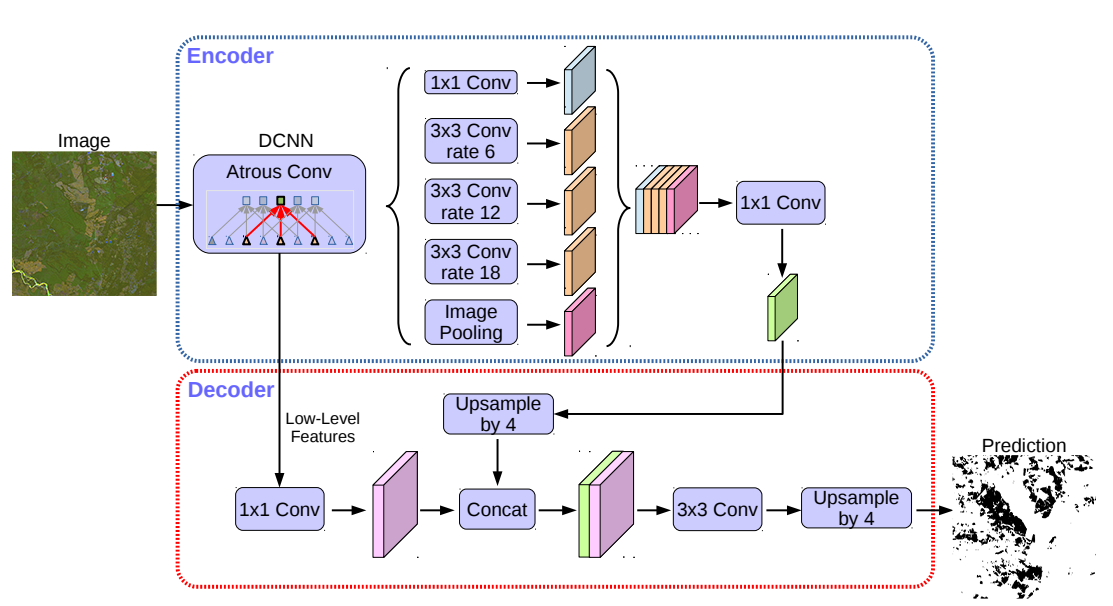
\includegraphics[width=\columnwidth]{model}
 \caption{Arquitectura DeepLabV3+ (Adaptado de \cite{chen2018})}
 \label{fig:model}
\end{figure}

Como se mencionó, la arquitectura de DeepLabV3+ se basa en un codificador que utiliza convolución \textit{atrous}, técnica heredada de DeepLabV3. Una innovación clave es la introducción de convoluciones \textit{atrous} separables, que descomponen las convoluciones en dos pasos: una convolución \textit{atrous} y una convolución punto a punto (1x1). Esto reduce significativamente los cálculos, manteniendo la eficiencia y la precisión en la segmentación.

El decodificador de DeepLabV3+ es crucial para recuperar información espacial perdida durante la codificación, mejorando la precisión de los detalles finos y los límites de los objetos. La aplicación de convoluciones separables en profundidad tanto en el módulo ASPP como en el decodificador aumenta la eficiencia computacional sin comprometer la precisión \cite{chen2018}.

Además, DeepLabV3+ mejora la segmentación en los límites de los objetos mediante técnicas avanzadas de decodificación, logrando una predicción precisa de píxeles. Su adaptabilidad a diferentes resoluciones de entrada permite ajustar el modelo según los recursos disponibles, haciéndolo aplicable desde dispositivos móviles hasta servidores.

La integración entre la red \textit{backbone} y el módulo decodificador es clave para su éxito. Mientras la \textit{backbone} actúa como codificador, el decodificador refina los resultados, especialmente en los límites de los objetos, utilizando características de bajo nivel para mejorar la precisión. Las convoluciones \textit{atrous} separables en el ASPP y el decodificador garantizan eficiencia sin sacrificar rendimiento.

\section{Desarrollo de la solución}

En esta sección se presenta un panorama completo del desarrollo de una solución para clasificar cultivos de palma de aceite en Colombia utilizando imágenes satelitales de Sentinel-1 y Sentinel-2. El proceso abarca desde el establecimiento del ambiente de desarrollo y las restricciones técnicas, hasta la construcción detallada del conjunto de datos, incluyendo la selección, el procesamiento de imágenes satelitales y su etiquetado. Asimismo, se describe el enriquecimiento del conjunto de datos mediante técnicas de aumentación, junto con la implementación y validación del modelo de aprendizaje profundo. Se enfatizan las estrategias empleadas para garantizar la precisión y efectividad del sistema en la identificación y clasificación de plantaciones de palma aceitera en Colombia.

\subsection{Ambiente de desarrollo, datos y restricciones}

El ambiente de desarrollo consistió en una máquina con sistema operativo Ubuntu, equipada con una tarjeta gráfica de 16 GB de VRAM y 16 GB de RAM. Este entorno fue seleccionado por su compatibilidad y rendimiento con herramientas de Deep Learning. Se utilizó Python como lenguaje de programación principal, junto con la librería PyTorch para el desarrollo y entrenamiento de los modelos. Entre las restricciones identificadas se encontraron limitaciones de memoria y tiempo de procesamiento, las cuales fueron mitigadas mediante técnicas de optimización de modelos y un uso eficiente de los recursos.

\subsection{Construcción del conjunto de datos}

\subsubsection{Preprocesamiento de Imágenes}

El preprocesamiento de las imágenes de los satélites Sentinel-1 y Sentinel-2 fue un paso crucial en la construcción del conjunto de datos, basado en la adaptación de la composición presentada por \cite{descals2021}. El proceso comenzó con la selección y descarga de imágenes desde Google Earth Engine (GEE). Para el Sentinel-1, se empleó el radar de apertura sintética (SAR) en modo Ground Range Detected (GRD), que ofrece una resolución temporal de 12 días en órbitas ascendentes y descendentes. Las imágenes correspondían a la modalidad de Interferometric Wide Swath y fueron procesadas a una resolución espacial de 10 metros. 

Un aspecto clave del preprocesamiento fue la corrección del ángulo de incidencia local (LIA), esencial para ajustar las imágenes de radar ante variaciones topográficas y de orientación. Tras realizar esta corrección, se calculó el valor mediano de las escenas de radar para la segunda mitad del año 2019, tanto para las órbitas ascendentes como descendentes. Finalmente, se generó un compuesto final promediando estos dos conjuntos de imágenes, representando ambas órbitas.

Este meticuloso preprocesamiento fue esencial para garantizar la calidad y precisión de los datos utilizados, asegurando una representación adecuada de las plantaciones de palma aceitera. Para el Sentinel-2, se utilizó específicamente la banda 4, conocida como la banda roja, con una longitud de onda central de 665 nm y una resolución espacial de 10 metros. Esta banda fue seleccionada por su alta utilidad en la identificación de plantaciones de palma aceitera, especialmente en plantaciones industriales. Su capacidad para ofrecer un alto contraste en la reflectancia entre los caminos dentro de las plantaciones y las áreas circundantes facilita la identificación de los caminos, un elemento crucial para diferenciar plantaciones industriales de pequeños propietarios. La elección de esta banda se debe también a que, en el espectro del infrarrojo cercano, la dispersión de luz alta dificulta la identificación de caminos en otras bandas, como la banda 8.

Por otro lado, para el Sentinel-1 se utilizó el modo Ground Range Detected (GRD) del radar de apertura sintética (SAR), procesado en la modalidad de Interferometric Wide Swath con una resolución espacial de 10 metros. Los datos del Sentinel-1, que operan en la banda C del espectro de microondas, son especialmente valiosos para detectar y clasificar características de la superficie terrestre, incluida la vegetación. Este radar proporciona datos confiables independientemente de las condiciones climáticas o de la iluminación, lo que lo hace ideal para monitorear extensas áreas de plantaciones de palma aceitera. Además, los datos de Sentinel-1 fueron procesados aplicando una corrección del ángulo de incidencia local (LIA), y se calculó el valor mediano de las escenas ascendentes y descendentes de la segunda mitad de 2019. Finalmente, se generó un compuesto final promediando ambas órbitas.

\subsubsection{Etiquetado de Imágenes}

El proceso de etiquetado de imágenes fue un paso fundamental para el entrenamiento y la predicción utilizando modelos de segmentación semántica. Este proceso incluyó varias etapas, detalladas a continuación:

\begin{itemize} 

    \item \textit{Establecimiento del Tamaño de las Imágenes:} Las imágenes utilizadas para el etiquetado y el entrenamiento del modelo debían tener un tamaño uniforme. Basándose en el trabajo de \cite{descals2021}, se definió un tamaño de entrada de 1000 x 1000 píxeles, correspondiente a un área de 10 x 10 km en imágenes con una resolución de 10 metros.

    \item \textit{Selección de Imágenes de Satélite:} Para el etiquetado, se utilizó la composición descrita en la etapa de preprocesamiento, correspondiente a un periodo semestral de imágenes de Sentinel-1 y Sentinel-2.

    \item \textit{Etiquetado:} El etiquetado de las imágenes se realizó utilizando los datos proporcionados por \cite{descals2021} en las zonas seleccionadas. Además, las máscaras de etiquetado de pequeños agricultores e industriales se unificaron en una única categoría.

\end{itemize}

\subsubsection{Aumento de Datos}

El proceso de aumento de datos se enfocó en generar un conjunto de datos de entrenamiento más diverso a partir del conjunto original, una técnica especialmente útil cuando el tamaño del conjunto de datos de entrenamiento es limitado. En este estudio, se aplicaron transformaciones afines a los datos de entrenamiento originales, específicamente la rotación de imágenes. Las imágenes fueron rotadas 90 grados en el sentido de las agujas del reloj.

El uso de transformaciones afines como la rotación es una práctica común en estudios de teledetección y aprendizaje profundo. Estas técnicas han demostrado mejorar la precisión de los modelos al crear un conjunto de datos de entrenamiento que representa de manera más efectiva la variabilidad y las diferentes orientaciones que pueden encontrarse en imágenes reales.

\subsection{Implementación del modelo}

El modelo acepta como entrada imágenes en formato PNG y genera salidas en el mismo formato, con una resolución de 1000x1000 píxeles. Posteriormente, estas salidas se convierten en imágenes en formato TIFF, incorporando georreferenciación y una máscara de salida proporcionada por el modelo. Para implementar la arquitectura DeepLabV3+, propuesta originalmente por \cite{chen2018}, se utilizó la biblioteca \texttt{segmentation\_models} de PyTorch. El modelo fue configurado con el codificador \texttt{timm-mobilenetv3\_large\_100}, preentrenado con el conjunto de datos ImageNet. Dado que el objetivo del modelo era clasificar la presencia o ausencia de palma de aceite, se definieron dos clases y se empleó la función de activación \textit{sigmoid}. La función de pérdida seleccionada fue la Entropía Cruzada Binaria (\textit{Binary Cross Entropy} - BCE), ideal para tareas de clasificación binaria.

El entrenamiento del modelo se llevó a cabo durante 20 épocas, evaluando y registrando las métricas especificadas en la sección 6.4.1 en cada iteración. Se guardó el modelo con el mejor rendimiento en cada época. El tamaño de lote (\textit{batch size}) se estableció en 7, optimizando el uso de los recursos computacionales disponibles. El conjunto de datos utilizado para el entrenamiento y la validación del modelo incluyó 270 imágenes, de las cuales el 70\% (189 imágenes) se asignaron al conjunto de entrenamiento, mientras que el 30\% restante (81 imágenes) se destinaron al conjunto de validación. Esta distribución equilibrada garantizó un entrenamiento eficiente y una validación precisa del modelo.

\subsection{Validación del modelo}

\subsubsection{Métricas}

Para garantizar una evaluación integral y precisa del modelo, se seleccionaron cuatro métricas clave: precisión (\textit{accuracy}), sensibilidad (\textit{recall}), precisión (\textit{precision}) y la puntuación F1 (\textit{f1-score}). Cada una de estas métricas ofrece una perspectiva única para analizar el rendimiento del modelo. Su combinación proporciona una visión holística y equilibrada, evaluando no solo la capacidad del modelo para clasificar con exactitud, sino también su eficiencia en identificar casos relevantes y minimizar falsos positivos.

\subsection{Validación de los resultados}

Para validar el modelo, se seleccionaron varias zonas dentro del territorio colombiano, elegidas por su relevancia agrícola y la diversidad de cultivos presentes, incluyendo, de manera prominente, plantaciones de palma de aceite. Esta selección permitió evaluar de manera efectiva el rendimiento del modelo en diferentes escenarios y condiciones ambientales, lo cual es esencial para asegurar su robustez y adaptabilidad.

Como parte del proceso de validación, se realizaron evaluaciones visuales utilizando el software QGIS \cite{QGIS_software}. Esta herramienta de Sistemas de Información Geográfica (SIG) permitió inspeccionar detalladamente las predicciones del modelo sobre los cultivos analizados. La evaluación visual en QGIS consistió en comparar las imágenes generadas por el modelo con las imágenes satelitales originales y los datos existentes sobre la ubicación y extensión de los cultivos en las zonas de estudio. Este enfoque no solo permitió medir la precisión general del modelo, sino también identificar sus limitaciones y áreas de mejora potencial, como la diferenciación entre tipos de cultivo y la precisión en la detección de los límites de las plantaciones.

\section{Pruebas y Resultados}

El modelo seleccionado, que demostró la mayor eficacia, se basó en la arquitectura MobileNet V3. Esta red neuronal convolucional fue elegida como la red troncal del modelo debido a su capacidad para operar eficientemente en dispositivos con recursos limitados, sin comprometer significativamente el rendimiento. Los resultados obtenidos son altamente prometedores, como se evidencia en las métricas de rendimiento del modelo. El modelo alcanzó una precisión global del 98.37\%, superando métodos tradicionales como SVM y Random Forest (precisión del 96\% según  \cite{diaz2023} ). Esto implica que el modelo es capaz de clasificar correctamente más del 98\% de las imágenes probadas, una métrica particularmente importante en aplicaciones prácticas donde la fiabilidad de la clasificación es crítica para el análisis posterior.

El \textit{recall} obtenido fue de 0.9914, reflejando la alta sensibilidad del modelo en la detección de las regiones con presencia de palma de aceite. En términos prácticos, esto significa que el modelo identificó correctamente el 99.14\% de todas las áreas relevantes en el conjunto de datos. Esta tasa de detección es crucial en estudios de cobertura de tierra, donde la omisión de áreas significativas puede llevar a conclusiones erróneas.

En cuanto a la precisión (\textit{precision}), el modelo alcanzó un 99.04\%, indicando que, de las regiones clasificadas como palma de aceite, el 99.04\% efectivamente correspondían a dichos cultivos. Esta alta precisión es indispensable para minimizar los falsos positivos, una métrica especialmente relevante cuando se toman decisiones de gestión de tierras basadas en los datos de clasificación.

Finalmente, el \textit{F1-score} del modelo fue de 0.9909, revelando un equilibrio casi perfecto entre precisión y \textit{recall}. Esto sugiere que el modelo no solo es altamente confiable en la identificación de áreas de palma de aceite, sino que también mantiene una baja tasa de falsos positivos y negativos, un aspecto fundamental para la integridad del análisis espacial. Estos resultados subrayan la eficacia del modelo MobileNet V3 para la detección de palma de aceite y su aplicabilidad potencial en la monitorización a gran escala de la agricultura y la gestión del uso de la tierra.

\begin{figure*}[t]
 \centering
 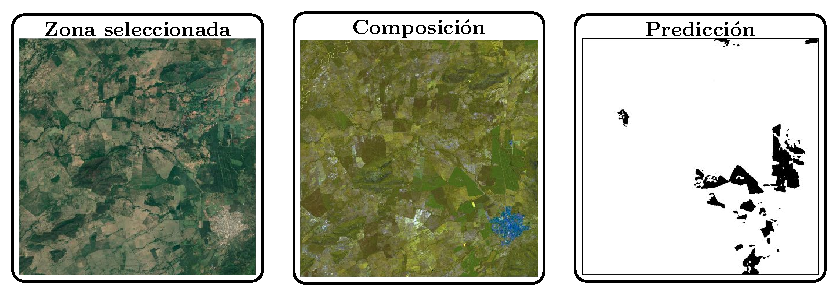
\includegraphics[width=\textwidth]{example_selected_zone}
 \caption{Ejemplo de predicción del modelo sobre un área con cultivos}
 \label{fig:example_selected_zone}
\end{figure*}

En la Figura \ref{fig:example_selected_zone} se muestra una zona seleccionada de 10x10 km en Colombia, seguida de la composición de Sentinel-1 y Sentinel-2. Finalmente, se presenta la salida del modelo, donde la clase 1, representada en negro, indica las áreas clasificadas como palma de aceite, mientras que las zonas en blanco en la máscara corresponden a las áreas donde el modelo identifica que no hay palma de aceite.

\begin{figure*}[t]
 \centering
 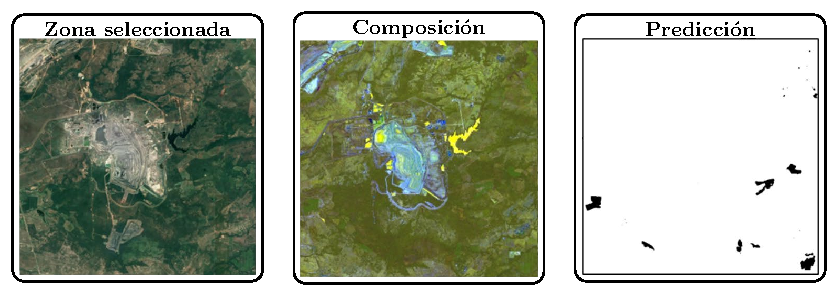
\includegraphics[width=\textwidth]{example_few_crops}
 \caption{Ejemplo de predicción del modelo sobre un área con pocos cultivos}
 \label{fig:example_few_crops}
\end{figure*}

En la Figura \ref{fig:example_few_crops} se observa una zona de explotación minera, que en la composición adquiere un color celeste. También se identifica un cuerpo de agua, representado con un color amarillo en la composición. Por otro lado, las plantaciones de palma de aceite se distinguen por un color verde característico. En esta zona seleccionada, los cultivos de palma de aceite son escasos, lo que explica que el color verde no sea predominante en la imagen. En la máscara predicha por el modelo, se puede apreciar que las áreas con plantaciones de palma de aceite se clasifican correctamente.

\begin{figure*}[t]
 \centering
 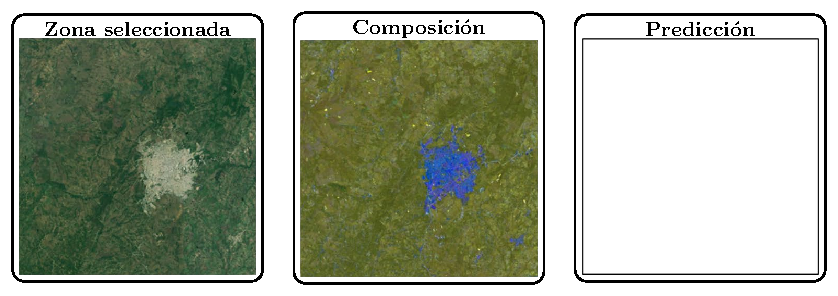
\includegraphics[width=\textwidth]{example_without_crops}
 \caption{Ejemplo de predicción del modelo sobre área sin cultivos}
 \label{fig:example_without_crops}
\end{figure*}

En la Figura \ref{fig:example_without_crops} se muestra una zona seleccionada donde no hay presencia de palma de aceite y, además, se encuentra una área metropolitana. En este caso, se observa que el modelo genera una máscara completamente blanca, lo que indica que clasifica correctamente la ausencia de cultivos de palma de aceite en esta zona.

\begin{figure*}[t]
 \centering
 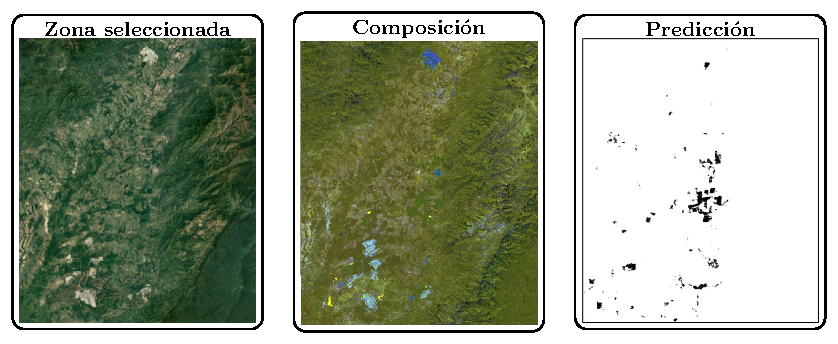
\includegraphics[width=\textwidth]{full_prediction}
 \caption{Predicción del modelo sobre toda la zona seleccionada}
 \label{fig:full_prediction}
\end{figure*}

En la Figura \ref{fig:full_prediction} se presenta la zona seleccionada en su totalidad, que incluye áreas metropolitanas, bosques, diversas plantaciones de otros cultivos, zonas rocosas y una gran diversidad de flora. A continuación, se muestra la predicción, donde las áreas en negro representan las regiones identificadas por el modelo como contenedoras de palma de aceite, mientras que las áreas en blanco indican la ausencia de este cultivo según la clasificación del modelo.

\begin{figure}
 \centering
 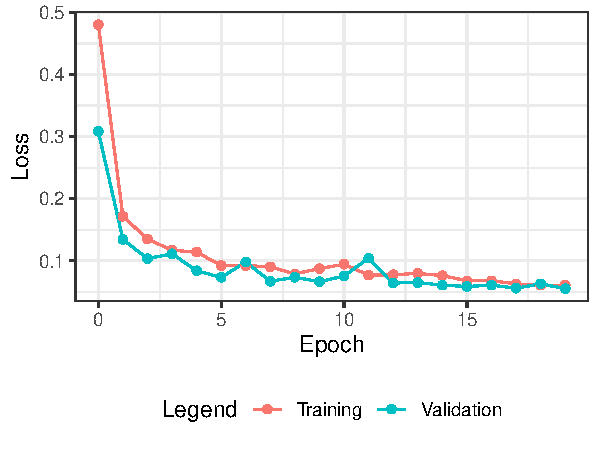
\includegraphics[width=\columnwidth]{loss}
 \caption{Gráfica de perdida (loss)}
 \label{fig:loss}
\end{figure}

\begin{figure}
 \centering
 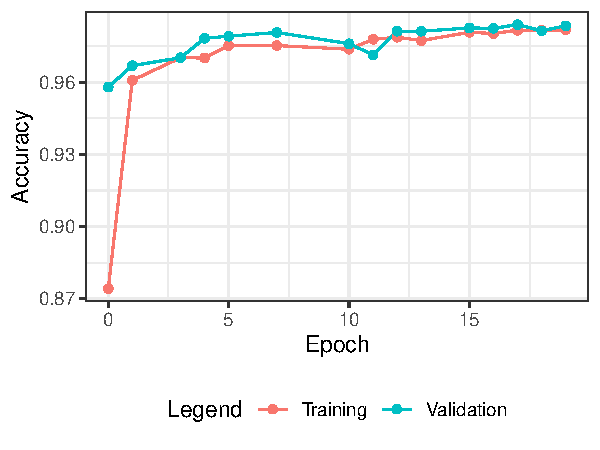
\includegraphics[width=\columnwidth]{accuracy}
 \caption{Gráfica de exactitud (accuracy)}
 \label{fig:accuracy}
\end{figure}

En el gráfico mostrado en la Figura \ref{fig:loss}, se observa la pérdida durante las etapas de  entrenamiento y validación. La pérdida disminuye rápidamente durante las primeras épocas, para luego estabilizarse, lo que sugiere que el modelo alcanzó un punto de convergencia de manera eficiente. De manera similar, en el gráfico \ref{fig:accuracy}, las líneas representan la precisión de entrenamiento y validación, ambas alcanzando valores superiores al 90\% y manteniéndose relativamente constantes después de las primeras épocas, lo que indica un buen ajuste del modelo.

\begin{figure}
 \centering
 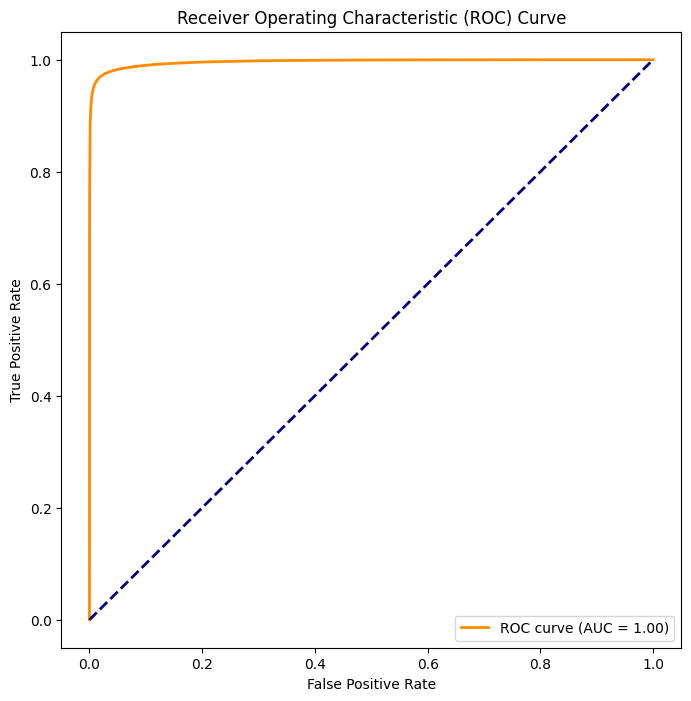
\includegraphics[width=0.8\columnwidth]{roc}
 \caption{Curva ROC del modelo}
 \label{fig:roc}
\end{figure}

La Figura \ref{fig:roc} muestra la Curva Característica de Operación del Receptor (ROC) con un área bajo la curva (AUC) de 1.00. La curva ROC, representada por una línea naranja, se adhiere perfectamente al borde superior izquierdo del gráfico, lo que indica un rendimiento excepcional del modelo. Esto demuestra una tasa de verdaderos positivos del 100\% en todos los umbrales de clasificación, mientras que la tasa de falsos positivos permanece en cero. El gráfico también incluye una línea punteada azul que representa el rendimiento de un clasificador aleatorio, lo que resalta aún más la superioridad del modelo evaluado.

Por último, al comparar este modelo con el presentado por \cite{diaz2023}, se observa que dicho estudio utilizó una variedad de algoritmos de aprendizaje automático más tradicionales, como regresión logística, Random Forest, SVM y XGBoost. Aunque estos métodos son eficaces y versátiles, no son tan específicos como los modelos de Deep Learning para tareas detalladas de segmentación de imágenes. Además, dicho análisis incorporó índices de vegetación y variables de textura, lo que enfatiza aspectos específicos de la vegetación y el terreno. Aunque esta metodología es útil, posiblemente no captura la gama completa de características obtenibles con el enfoque basado en Deep Learning. La precisión del modelo en dicho trabajo fue ligeramente inferior, con un 96\%, lo que sugiere que los enfoques tradicionales de aprendizaje automático siguen siendo efectivos para tareas de clasificación detalladas, aunque menos precisos que los métodos avanzados de Deep Learning.

\section{Conclusiones y Trabajos futuros}
Este estudio demuestra la eficacia del uso de técnicas avanzadas de Deep Learning para la clasificación de cultivos de palma de aceite en Colombia, integrando datos satelitales de Sentinel-1 y Sentinel-2. El modelo propuesto, basado en DeepLabV3+ y MobileNet V3, alcanzó una precisión global del 98.37\%, superando significativamente los métodos tradicionales. Estos resultados destacan la capacidad del enfoque para manejar desafíos complejos como la integración de datos radar y ópticos, y su robustez ante condiciones como la cobertura de nubes.

Sin embargo, se identificaron limitaciones, particularmente en la detección de áreas recientemente despejadas y plantaciones jóvenes. Esto sugiere la necesidad de incorporar datos adicionales que reflejen mejor la variabilidad en las etapas de desarrollo de las plantaciones. Además, técnicas como la rotación de imágenes han demostrado ser esenciales para enriquecer los datos de entrenamiento y mejorar la eficacia del modelo, especialmente en regiones con conjuntos de datos limitados.

En comparación con enfoques tradicionales, como los basados en índices de vegetación y algoritmos de aprendizaje automático, el modelo de Deep Learning exhibe una superioridad notable en tareas específicas de clasificación y segmentación de imágenes agrícolas. Este trabajo subraya el potencial de estas herramientas para transformar la agricultura de precisión, no solo en Colombia, sino también en otros contextos globales.

Para futuros estudios, se recomienda ampliar el conjunto de datos, incluir más variedades de cultivos y explorar análisis temporales utilizando series de imágenes satelitales. Asimismo, sería valioso investigar cómo las condiciones climáticas y estacionales afectan la precisión del modelo, además de priorizar la interpretabilidad de los resultados para fomentar su adopción en aplicaciones del mundo real. Estas iniciativas fortalecerán aún más el impacto de las tecnologías de Deep Learning en la sostenibilidad y gestión agrícola.


\bibliographystyle{IEEEtran}
\bibliography{IEEEabrv, main}

\end{document}
